\documentclass{beamer}

\usepackage[T1]{fontenc}
\usepackage[utf8]{inputenc}
\usepackage{lmodern}
\usepackage{graphicx}
\usepackage[absolute,overlay]{textpos}
\usepackage{multicol}
\usepackage{listings}
\usepackage{svg}

%% Beamer customization--------------------------------------------------------

\usepackage{xcolor}


\usepackage{tikz}

\usetheme{Warsaw}

%% Themes
% Outer themes
\useoutertheme{shadow}
% Rounded boxes and shadows
\useinnertheme[shadow=true]{rounded}
% Solid \item symbols
\useinnertheme{circles}

%% Custom colors
\definecolor{rltgreen}{rgb}{0,0.5,0}
\definecolor{pasteur}{RGB}{0,90,154}
\setbeamerfont{block title}{size={}}
\setbeamercolor{structure}{fg=pasteur}
\setbeamercolor{item}{fg=pasteur}


%Color of title
\setbeamertemplate{frametitle}
{    \nointerlineskip
    \begin{beamercolorbox}[sep=0.3cm,ht=1.8em,wd=\paperwidth]{frametitle}
        \vbox{}\vskip-2ex%
        \strut\insertframetitle\strut
        \vskip-0.8ex%
    \end{beamercolorbox}
}
% Hide navigation symbols
\setbeamertemplate{navigation symbols}{}

%% Title block
\setbeamercolor*{title}{use=structure,fg=white,bg=pasteur}

\makeatletter

%% Top infolines
\setbeamertemplate{headline}{%
\leavevmode%
  \hbox{%
    \begin{beamercolorbox}[wd=\paperwidth,ht=2.5ex,dp=1.125ex]{palette quaternary}%
    \insertsectionnavigationhorizontal{\paperwidth}{}{\hskip0pt plus1filll}
    \end{beamercolorbox}%
  }
}


%% Define Snakemake -----------------------------------------------------------

\definecolor{eclipseBlue}{RGB}{42,0.0,255}
\definecolor{eclipseGreen}{RGB}{63,127,95}
\definecolor{eclipsePurple}{RGB}{127,0,85}

\lstset{language=Python}
\lstset{
    basicstyle=\scriptsize\ttfamily,
    morekeywords={rule, output, shell, params, run, configfile, temp, log},
    showstringspaces=false,
    commentstyle=\color{eclipseGreen}, % style of comments
    keywordstyle=\color{eclipsePurple}, % style of keywords
    stringstyle=\color{eclipseBlue}, % style of strings
}



%% Set up title ---------------------------------------------------------------

\title[Sequanix]{Sequanix: a GUI for snakemake pipelines}
\author[T. Cokelaer]{Thomas Cokelaer}
\institute{Institut Pasteur}
\date{Dec 15th 2017, Snakemake Day, Amsterdam}


\AtBeginSection[]{
  \begin{frame}
  \vfill
  \centering
  \begin{beamercolorbox}[sep=8pt,center,shadow=true,rounded=true]{title}
    \usebeamerfont{title}\insertsectionhead\par%
  \end{beamercolorbox}
  \vfill
  \end{frame}
}

\begin{document}

%% Title slide ----------------------------------------------------------------

\begin{frame}[plain]
    \titlepage
    \begin{textblock*}{5cm}(4.5cm,0.3cm)
        
\includegraphics[scale=0.09]{images/Institut_Pasteur.png}
    \end{textblock*}
\end{frame}

%% Slides ---------------------------------------------------------------------

\begin{frame}
\frametitle{Motivation}
\begin{block}{Jan 2015: Needed to provide NGS pipelines to Biomics sequencing platform 
https://research.pasteur.fr/en/team/biomics/ (Institut Pasteur)}
 \begin{itemize}
  \item Genomics: QC + variant calling + de-novo
  \item Transcriptomics: RNA-seq + ChIP-seq 
  \item Metagenomics
  \item Illumina but also Pacbio long reads technologies
 \end{itemize}
 %\includegraphics{images/genetic_strand.png}
 %\includegraphics{images/strand.png}
\end{block} 
\end{frame}



\begin{frame}
\frametitle{How ?}

\begin{columns}
\begin{column}{1.5cm}

\includegraphics[height=0.2\textheight]{images/logo_python.png} 
\end{column}
\begin{column}{9cm}
a glue language, a scientific language
\end{column}
\end{columns}


\rule{\textwidth}{1pt}


\begin{columns}
\begin{column}{1.5cm}

\includegraphics[height=0.2\textheight]{images/logo_snakemake.png}
\end{column}
\begin{column}{9cm}
a pipeline 
framework mixing Python and Makefile \\
{\footnotesize \textcolor{blue}{\textit{Köster, Johannes and Rahmann, Sven. 
Snakemake - A scalable 
bioinformatics workflow engine. Bioinformatics 2012.}}}
\end{column}
\end{columns}

\rule{\textwidth}{1pt}


\begin{columns}
\begin{column}{1.5cm}

\includegraphics[height=0.2\textheight]{images/exe.png}
\end{column}
\begin{column}{9cm}
Dedicated standalone such as genome coverage characterisation or a graphical 
user interface for Snakemake pipelines (Sequanix).
%{\footnotesize \textcolor{blue}{\textit{D. Desvillechabrol, C. 
%Bouchier, S. Kennedy, T. Cokelaer Detection and characterization of low 
%and high genome coverage regions .... BioRxiv 
%https://doi.org/10.1101/092478 }}. Submitted to GigaScience journal }
\end{column}
\end{columns}



\end{frame}



\begin{frame}
\frametitle{Pipeline example: variant calling}
\centering
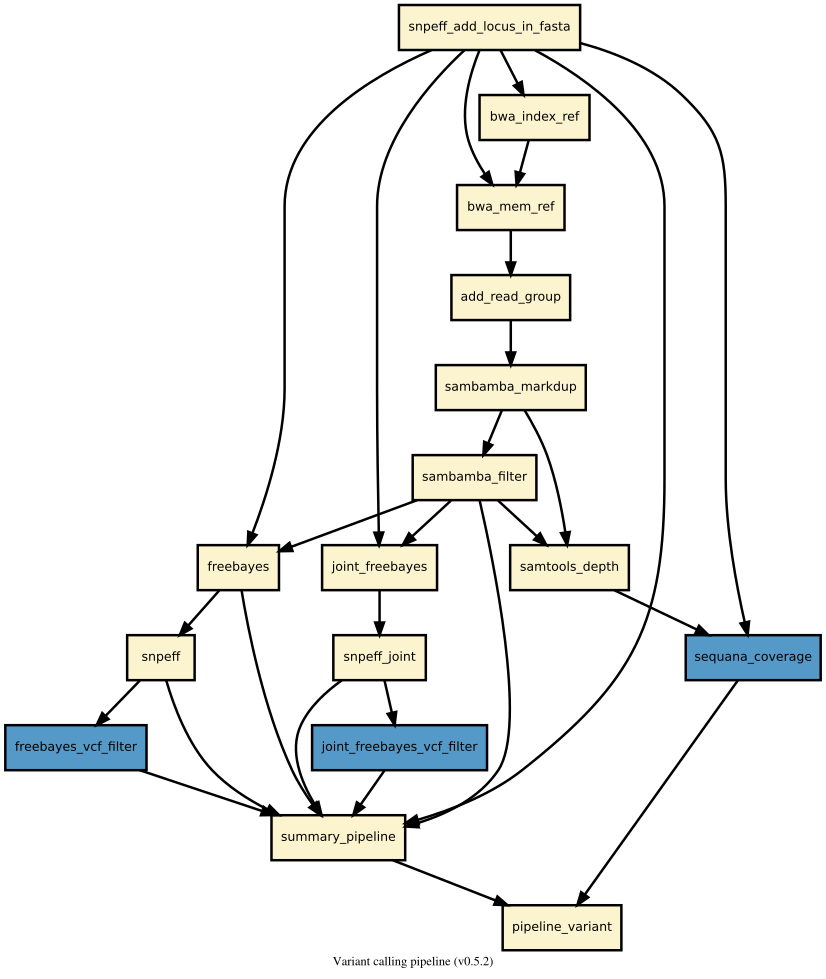
\includegraphics[height=0.8\textheight,
width=\textwidth]{./images/variant_calling_dag.png}
\end{frame}


\begin{frame}[fragile]
\frametitle{Complex pipeline $\rightarrow$ complex configuration file}

\begin{lstlisting}{python}
input_directory: "%(input_directory)s"
input_readtag: "%(input_readtag)s"
input_extension: "%(input_extension)s"
input_pattern: "%(input_pattern)s"
input_samples:
    file1: "%(file1)s"
    file2: "%(file2)s"

bwa_mem_ref:
    reference: "%(reference)s"
    index_algorithm: 'is'
    options: '-T 30'
    threads: 2
    tmp_directory: './tmp/'
\end{lstlisting}
\end{frame}

\begin{frame}[fragile]
\frametitle{Execution}

\begin{lstlisting}[basicstyle=\ttfamily\large]
snakemake -s gc_minimalist.rules
\end{lstlisting}

\rule{\textwidth}{1pt}

More options if a configuration file is required, or execution is on a cluster, 
or \dots something goes wrong.
\end{frame}


\begin{frame}
\frametitle{Practical considerations}

\begin{block}{Sequanix}
\begin{itemize}
 \item Users do not want to see the Snakefile
 \item Developers do not want users to see the Snakefile
 \pause
 \item Users do not want to edit the configuration file manually
 \item Developers do not want users to edit the configuration file manually
 \pause
 \item We want a GUI that works on a local computer or on clusters.
 \pause
 \item Sequana developers want to expose their pipelines dynamically
 \pause
 \item What about other Snakemake pipelines ? 
\end{itemize}
\end{block}
\end{frame}


\section{Sequanix, a GUI for snakemake pipelines}
\begin{frame}{GUI to simplify the usage of snakemake}
    \begin{columns}
        \begin{column}{0.5\textwidth}

            \only<1>{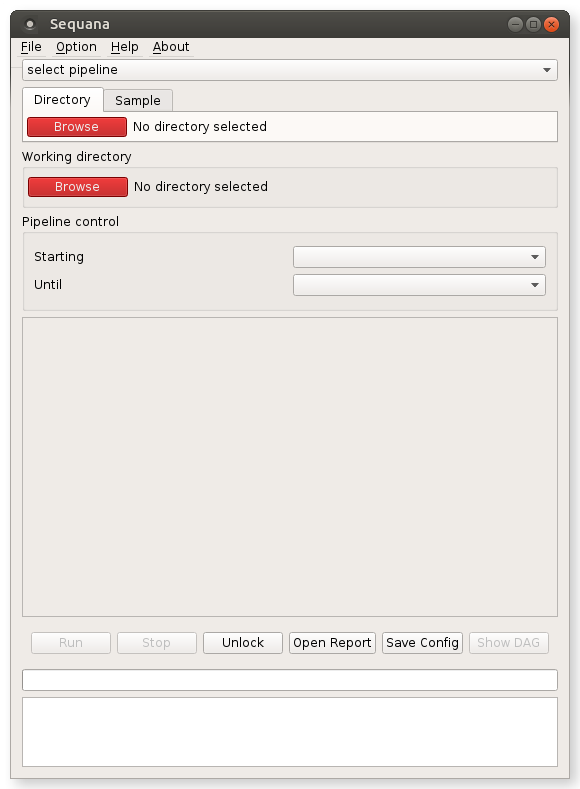
\includegraphics[scale=0.25]{../../images/sequana_init}}

            \only<2>{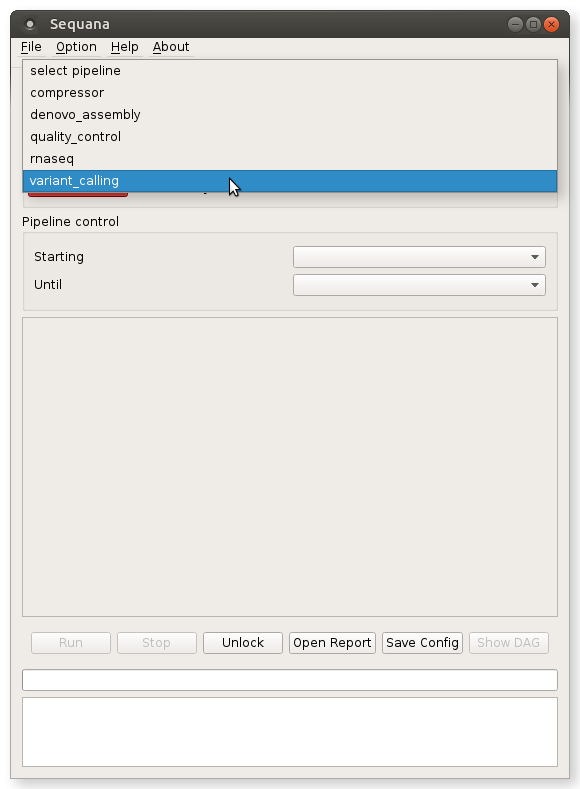
\includegraphics[scale=0.25]{../../images/choose_pipeline}}

            \only<3>{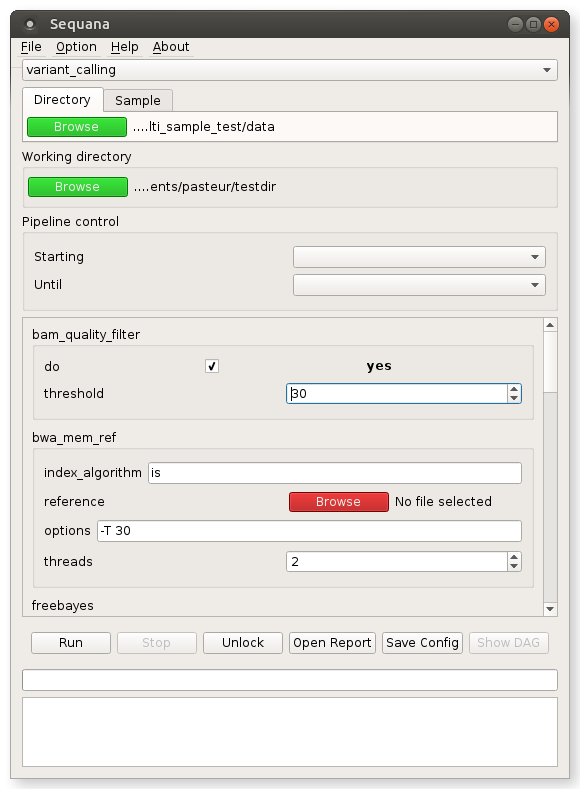
\includegraphics[scale=0.25]{../../images/choose_input_output}}

            \only<4>{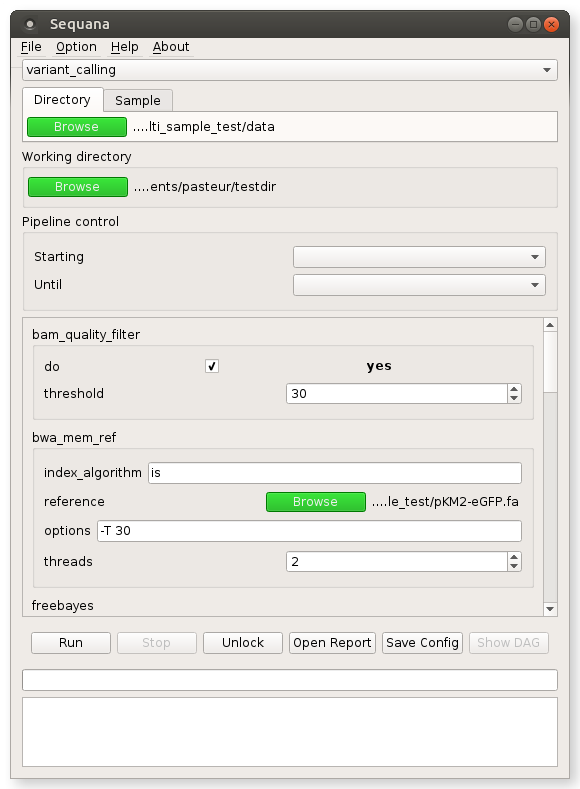
\includegraphics[scale=0.25]{../../images/sequana_pipeline}}

            \only<5>{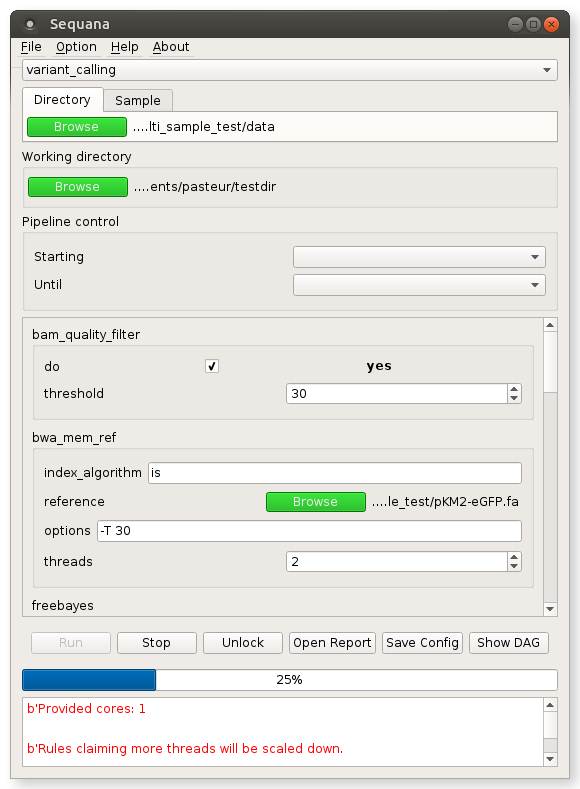
\includegraphics[scale=0.25]{../../images/sequana_running}}

            \only<6>{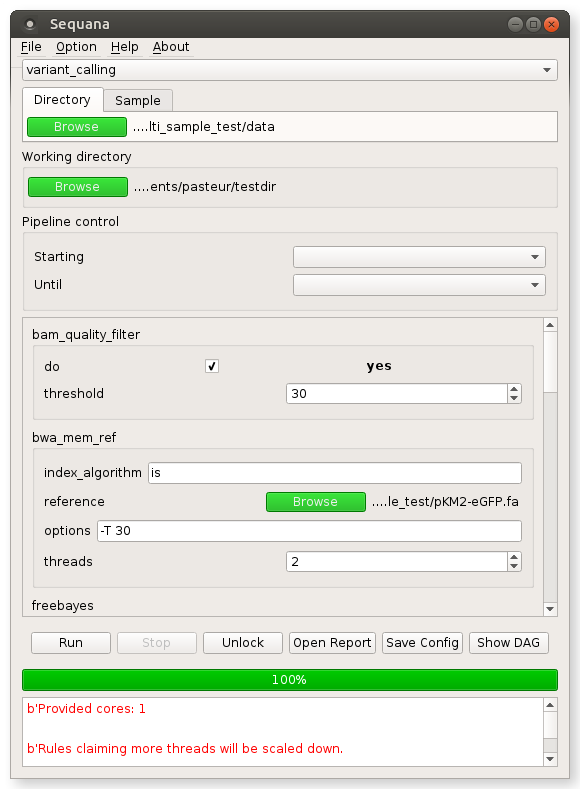
\includegraphics[scale=0.25]{../../images/sequana_finish}}

        \end{column}
        \begin{column}{0.5\textwidth}
            \only<1>{
                \begin{itemize}
                    \item Interface developed with PyQT5 and python
                    \item Wrap our snakemake pipelines to ease the usage
                    \item Usable on our cluster, which allows X11
                \end{itemize}
            }
            \only<2-6>{
            \begin{enumerate}
                \item<2-6> Choose a pipeline
                \item<3-6> Set input and output
                \item<4-6> Fill the config formular
                \item<5-6> Run the pipeline
                \item<6> Finished !
            \end{enumerate}
            }
        \end{column}
    \end{columns}
\end{frame}




\begin{frame}
  \frametitle{Snakemake options available}
  \centering
   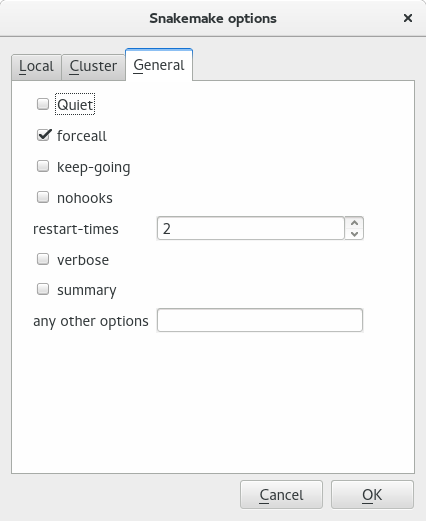
\includegraphics[height=0.8\textheight,width=0.5\textwidth]
   {./images/snakemake_general.png}
\end{frame}


\begin{frame}
\frametitle{Tooltips for each configuration config section}
\centering
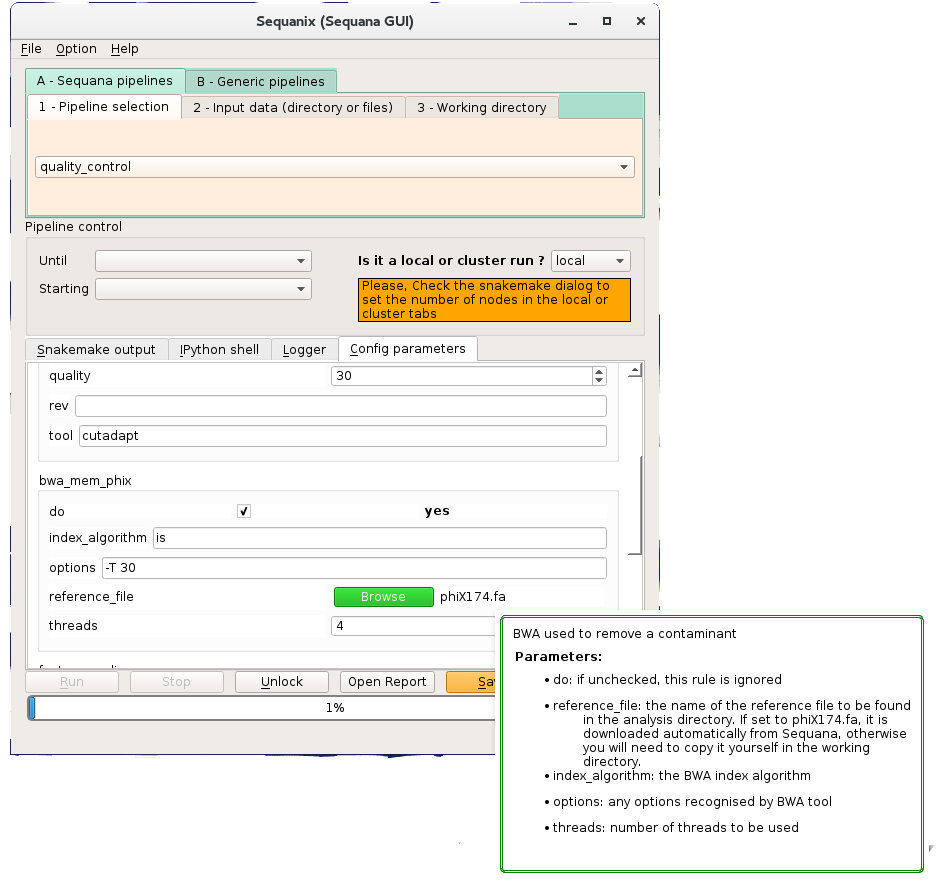
\includegraphics[height=0.8\textheight, width=0.65\textwidth]{./images/dialog_tooltip.png}
\end{frame}



\begin{frame}
\frametitle{Reference} 
 
\textbf{Sequanix: A Dynamic Graphical Interface for Snakemake Workflows} 

\vspace{.5cm}

\textit{Dimitri Desvillechabrol, Rachel Legendre, Claire Rioualen, Christiane 
Bouchier, Jacques van Helden, Sean Kennedy, Thomas Cokelaer}

\vspace{.5cm}
 
https://www.biorxiv.org/content/early/2017/07/12/162701
 
\end{frame}



\section{Summary}

\begin{frame}
 \frametitle{Summary}

\begin{block}{Take home message}
    \begin{itemize}
        \item Sequanix was developed to provide a GUI dedicated to Sequana NGS pipelines
(http://sequana.readthedocs.io)
        \item We make it generic for any Snakemake pipelines
    \end{itemize}
\end{block}

\begin{block}{You like it ? Please, add a star on our github}
    https://github.com/sequana/sequana/stargazers
    \centering
\end{block}

\begin{block}{Acknowledgements}
 \begin{itemize}
  \item Dimitri Desvillechabrol (variant calling, Sequana, Sequanix)
  \item Rachel (Transcriptomics)
  \item M\'elissa Cardon (pacbio)
  \item Biomics users (Institut Pasteur)
 \end{itemize}
\end{block}

\end{frame}








\end{document}
